% % !TEX root = ./ApproximatingDOGs.tex

% \section{Controlling the granularity} \label{sec:user-control}

%%%%%%%%%%%%%% OUT %%%%%%%%%%%%%%%%




% While our algorithm is fully automatic, we do allow users to tailor the result to their needs. There is always a trade-off between the approximation accuracy and the number of patches of the piecewise developable result. The number of patches governs the assembly effort, for example,  which is something that our algorithm cannot define, as it is up to users' preferences. For some application scenarios (e.g., architecture) reduced assembly effort might be favorable, meaning that users would prefer a low number of patches. For other applications or fabrication techniques (e.g., flank milling), users might be more concerned with higher approximation accuracy, independent of the number of parts generated. To support this, our algorithm allows users to specify their preference on a high level. \figref{fig:granularity} shows the non-developable Lilium model approximated with 3 different levels of granularity, resulting in piecewise developable models with 6, 13, or 20 patches, respectively. 
% Users can specify the general granularity, which by default balances the approximation error and the number of patches. 
% They can also fix the number of patches or the approximation error independently, as we detail in the following.



% \begin{figure} [h!]
% \centering
% \noindent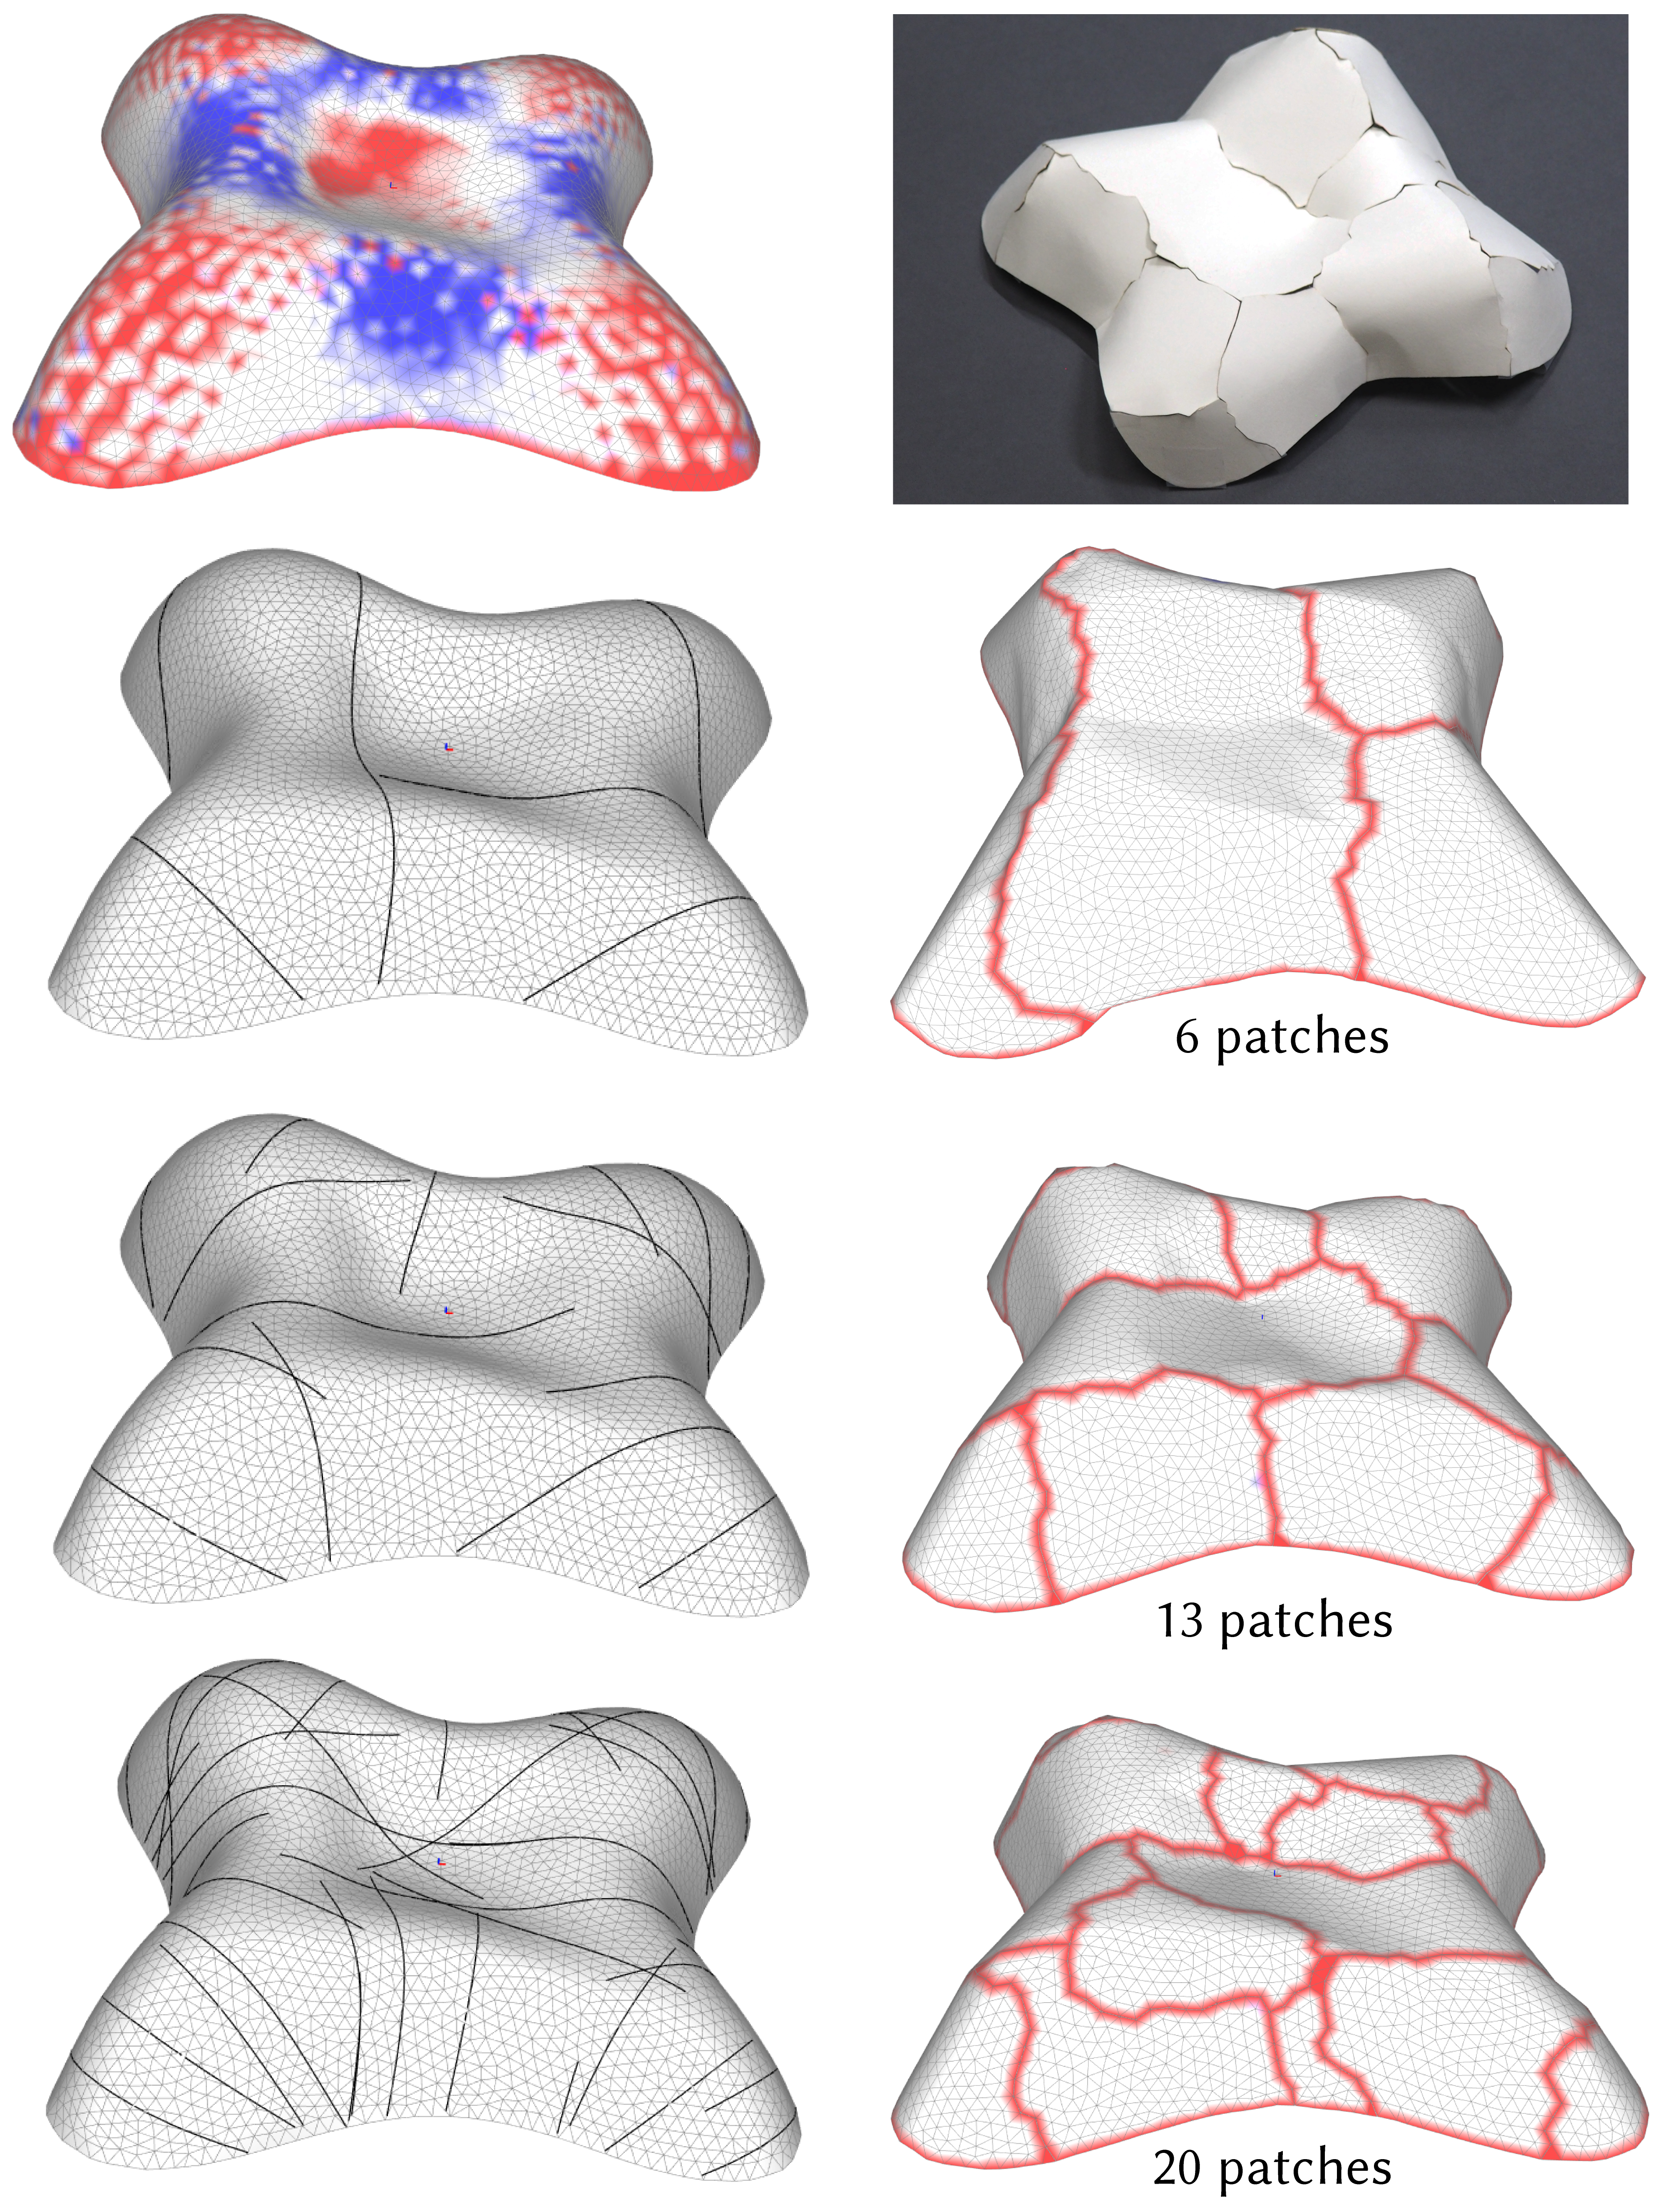
\includegraphics[width=\linewidth]{figures/FIG granularity 3x lilium grid-01.png}
% \caption{
% 	\AI{todo.}
% 	Our algorithm allows adapting the granularity of the resulting piecewise developable surface according to users' preferences. Naturally, fewer patches result in a higher approximation error. We show 3 versions of the same model, with 6, 13 and 20 patches and denote their Hausdorff distance $d_H$ and the total approximation error $\eps_\text{sum}$ as the sum of the per-vertex distance from $V_t$ to any point on the developable result. The metrics are relative to the shape's size, here bounding box diagonal is 28.8.\\
% 	\AI{- visual: remove mesh \& gauss from result, add error map, add used parameters of $ \lambda, \delta, \eps $.}\\
% 	\AI{- error values got lost! fix also in text}
% 	% \AI{add color scale, re-arrange image}
% 	\label{fig:granularity}}
% \end{figure}

% The granularity of the developable result is defined by 3 parameters, which we already discussed in the previous sections: 
% \begin{enumerate}
% 	\item $\lambda$, the penalty in the smoothness term of our geodesics selection, as it defines the number of DOG patches to approximate,
% 	\item $\delta_{\text{distance}}$, which defines how much the DOG patch can stretch to cover a larger surface, and
% 	\item $\eps_{\text{max}}$, the maximum per-vertex approximation error that defines areas considered as being uncovered.
% \end{enumerate}

% \todo{! show sensitivity to parameters here.}

% % \paragraph{Balanced granularity.}
% By default, our algorithm aims to balance the approximation error and the number of patches. The biggest influencing factor is the geodesics selection in our initialization procedure, governed by $\lambda$. This defines how many DOG patches are fitted to the target shape. A lower value results in more patches and therefore in a higher granularity. Conversely, a higher smoothness value results in lower granularity. 
% Based on the user-defined smoothness value, we automatically adapt the value of $\delta_{\text{distance}}$, where a higher value allows for more stretch and more deviation from the target surface. We adapt $\delta_{\text{distance}}$ relative to the average edge length $\overline{e}$ of the target $\target$. We interpolate $\delta_{\text{distance}}$ between $ 4 \overline{e} $ for low granularity and $ 0.9 \overline{e} $ for high granularity, as we empirically found good approximation results within these bounds. 
% The approximation error $\eps_{\text{max}}$ is an absolute threshold independent of the mesh resolution. The default value in our implementation is $0.8$. 

% The initial number of selected geodesics might not be the resulting number of piecewise developables, as additional patches are added for uncovered areas. 
% To control the number of developable parts, users can disable the approximation error $\eps_\text{max}$ by setting it very high such that no uncovered areas are detected. 
% Conversely, setting $\eps_\text{max}$ allows users to create results with a user-defined maximum approximation error since uncovered areas will be approximated until all are covered.

% % \paragraph{Specifying the number of patches.}
% % To force the algorithm to stick to n parts, we can disable the hole patching and set the outlier threshold <high> to allow for stretching and thus coverage with few patches.

% % \paragraph{Specifying the approximation error.} 
% % Enforcing a maximum approximation error is trickier. Mainly, we need to select geodesics until we get an approximation error of <2 * max. Error>. this is because the ruled surfaces are not precise and the DOG patches typically fit way better. Of course, the coverage threshold is then set to <max. Error * 0.8 or so>. At the Result step, we select (by lowering the smoothness) until we found an assignment with the desired max. Error, disregarding the number of patches.


% % \paragraph{}

% In \figref{fig:granularity}, we note that the error values of the version with 13 and 20 patches are very similar, considering that they differ by 7 patches. This suggests a pareto-optimal front that governs the tradeoff between number of patches and approximation error. While it is outside the scope of this paper, we think that investigating how this might relate to the surface properties of a shape is an interesting opportunity for future work.
